\documentclass[12pt]{article}
\usepackage[utf8]{inputenc}
\usepackage[russian]{babel}
\usepackage{graphicx}
\usepackage{subcaption}
\graphicspath{ {./images/} }


\begin{document}

\textit{\textbf{Задание 13.}}

\textit{Задана система булевых функций $f_1=10110110$ и $f_2=00110011$. Проверьте
данную систему на полноту. Выполнить полную проверку для обеих функций.}

\underline{Решение:}

Проверим выполнение теоремы Поста о полноте.

Класс $P_0$: Первый бит $f_1$ не 0, эта функция ноль не сохраняет, первый бит
функции $f_2$ – ноль, эта функция ноль сохраняет.

Класс $P_1$: Последний бит $f_1$ - 0, эта функция единицу не сохраняет,
последний бит функции $f_2$ – один, эта функция единицу сохраняет.

Класс $S$: Проведем проверку по схеме (делим каждую функцию пополам
и, двигаясь от центра проверим что все биты различны):

\begin{figure}[h]
        \captionsetup[subfigure]{labelformat=empty}
        \centering
        \begin{subfigure}{.32\textwidth}
                \centering
                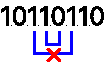
\includegraphics[width=1\linewidth]{13_1.pdf}
                \caption{Для $f_1$}
        \end{subfigure}
        \begin{subfigure}{.32\textwidth}
                \centering
                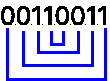
\includegraphics[width=1\linewidth]{13_2.pdf}
                \caption{Для $f_2$}
        \end{subfigure}
\end{figure}

Класс M: Разобьем каждую из функций пополам и проведем побитовое
сравнение полученных частей. Если функция монотонна, то каждый бит первой
половины должен быть «меньше или равен» соотвествующего бита второй
половины. Продолжаем этот процесс до конца.

\begin{center}
        \begin{tabular}{ |c|c| }
                \hline
                Для $f_1$: & Для $f_2$: \\
                \hline
                \underline{1}011 & 0011 \\
                \underline{0}110 & 0011 \\
				\hline
        \end{tabular}
\end{center}

Не выполняется в подчеркнутой позиции.

Класс L: для каждой функции построим полином Жегалкина (см.
задание 8). Получим:

$f_1=1 + z + yz + x + xy + xyz$ - не линейна, т.к. есть конъюнкции,

$f_2 = y$ - линейна, т.к. нет конъюнкций.

Сведем все результаты в таблицу:

\begin{center}
        \begin{tabular}{ |c|c|c|c|c|c| }
                \hline
                 & $P_0$ & $P_1$ & $S$ & $M$ & $L$\\
                \hline
                $f_1$ & - & - & - & - & -\\
				\hline
                $f_2$ & + & + & + & + & +\\
				\hline
        \end{tabular}
\end{center}

В каждом столбце есть «минус», следовательно условия теоремы Поста
выполняются! Данная система функций является полной!

\end{document}
